\chapter{计算机病毒的预防}

我们已经向读者介绍了病毒的概念和对于系统的实际病毒。已经种下潜在的毁灭性袭击的种子,所以适当的检查保护机制可以帮助抵御它。我们在这里研究计算机病毒的预防。

\section{基本的限制}

为了系统中的用户能够共享信息,必须存在一个信息路径可以让信息从一个用户传送到另一个用户。我们不区分用户和作为用户代理的程序,这是因为在任何计算机使用中程序总是作为用户的代理,而且我们忽略通过用户的秘密通道。假设有一个计算的图灵机模型,我们可以证明如果信息可以由用户通过图灵能力进行读取,那么它就可以被复制,复制后可以被视为一个图灵机磁带上的数据。


给定一个通用的系统,用户可以按照自己的希望使用自己具有的信息,并且传递这些他们认为合适的信息,可以清楚的看到,分享信息的能力是可传递的。也就是说,如果有一条从用户A到用户B的路径,还有一条从用户B到用户C的路径,那么在用户B有意或者不知情的合作下,存在从用户A到用户C之间的路径。


最后,可以用作数据和程序的信息之间没有本质的区别。这可以清楚的在翻译的情况下看出来,信息编辑成数据,并译作一个程序。实际上,信息只有在译出之后才有意义。

在一个信息可以被接受者译作一个程序的系统中,这种翻译可能导致如上所示的感染。如果存在分享,感染可以通过共享信息的解释进行传播。如果对信息流的传递性没有限制,那么从任何资源开始,信息可以到达信息流的传递闭包。共享、信息流的传递性和解释的普遍性使得在任何给定的资源的条件下,病毒可以传播到信息流的传递闭包。


显然,如果没有共享,就没有跨边界信息的传染,因此外部的信息不能解释,并且病毒不能在单个分区之外进行传播。这就是所谓的“隔离”。显然,系统中如果没有程序可以改变并且没有信息用于决策,那么系统不会被感染,这是因为感染需要解释信息的修正。我们称之为“固定一阶函数”系统。我们应该注意到,几乎任何具有实际效用的科学系统或开发环境需要解释的普遍性,如果我们希望从别人的工作中获益,那么隔离是不可接受的。然而,在有限的情况下可能存在病毒问题的解决办法。


\section{分区模型}

可以将限制信息流动的路径分为两类,一些将用户在传递条件下分割成适当的闭子集,另外一些则不进行分割。流量限制可以导致闭子集视为一个系统的分区并成孤立子系统。这让每一次感染限制在一个分区中。这是一个可行的预防手段,用于预防病毒在有限隔离下的完全占领,相当于给每个分区自己的计算机。


完整性模型\cite{5}提供一种策略,它可用于在传递性条件下将系统分割成封闭子集。在Biba模型中,一个完整性层次与所有信息都相关联。严格的完整属性是Bell-LaPadula属性的双重叠加;在一个给定的完整性水平下,没有用户可以读取一个完整性水平更低的对象,也不能写出一个完整性水平更高的对象。在Biba最初的模型中,读取和执行访问之间是有区别的,但是在没有限制信息解释的普遍性的条件下不能执行,这是因为一个高完整性的程序可以编写一个低完整性的对象,并且对其进行复制,然后读取低完整性的输入并且产生低完整性的输出。


如果完整性模型和Bell-LaPadula模型共存,一种有限隔离可以通过传递性将空间划分为有限的闭子集。如果相同的划分用于机制(高完整性与高安全性),孤立主义结果信息提升安全水平也提升了完整性水平,但这是不被允许的。当Biba模型的边界在Bell-LaPadula模型的边界内的时候,感染只能在一个给定的安全水平下从高完整性水平向低完整性水平扩散。最后,当Biba模型的边界在Bell-LaPadula模型的边界内的时候,感染只能在一个给定的安全水平下从低完整性水平向高完整性水平扩散。对应于低边界性和高边界性,实际上有9种不同的情况,但下面图形显示了其中的三个,这已经可以让大家充分理解了。


Biba的工作还包括另外两个完整性策略,“低水位标志”策略使得对于任何输入可以输出最低的完整性,以及“环”策略使得用户无法调用他们能够阅读的一切东西。前一个策略倾向于将所有信息转移到完整性水平较低处,而后者试图区别那些不能用广义解释的信息。


正如基于Bell-LaPadula模型的系统总是通过提高水平来使得所有信息转移到更高水平的安全性上,以此满足高水平的用户,而Biba模型倾向于通过减少最低传入结果的完整性将所有信息转移到较低的完整性水平上。我们也知道,一个精确系统的完整性是NP-完全问题(正如它的对偶是NP-完全的)。


最值得信赖的程序员(由定义)应该可以编写可以让大多数用户使用的程序。为了保证Bell-LaPadula策略,高水平用户无法编写由低水平的用户使用的程序。这意味着最信任的程序员必须是最低的安全级别的。这似乎是矛盾的。当我们把Biba和Bell-LaPadula模型联合起来的时候,我们发现产生的孤立主义保护我们免受病毒的攻击,但是不允许任何用户编写让整个系统使用的程序。但实际上,就像我们允许数据的加密或解密,把它从高安全水平转移到低安全性水平上,我们应该能够使用程序测试和验证将信息从低完整性水平转移到高完整性水平上。


另一个用于将系统分割成闭子集的常用的策略也用于典型的军事应用。这一策略将用户分类,每个用户只能访问他们的职责所需的信息。如果每一个用户在特定的时间只能一访问一个类别,系统可以避免跨类别边界病毒攻击,这是因为他们是孤立的。不幸的是,在目前的系统中,用户可以同时访问多个类别。在这种情况下,感染可以通过边界传播到信息流的传递闭包。


\section{流模型}

一些不通过传递性将系统分割成闭子集的策略,可以限制病毒传播的程度。“流距离”策略实现了通过记录数据流的距离(共享的数目)产生距离矩阵。输出信息的距离是输入信息的最大距离,并且共享信息的距离比信息共享之前的距离多一个。通过采用一个阈值使得在此之上的信息变得无法使用,以此引入保护。因此与距离8的文件共享一个距离为2的进程,可以将进程距离增加到9,并且任何进一步的输出将至少有这个距离。


“流列表”策略维护所有对每个对象有影响的用户。规则维护该列表,即输出流的流列表是所有输入的流列表的并(包括导致行动的用户)。保护需要采用决定可访问性的任意布尔表达式的形式流列表。这是一个非常通用的策略,可以通过选择合适的布尔表达式来表示任何上述策略。


在例子中,用户A只能获取由用户B和C或者用户B和D写的信息,但是不能获取单独由B或者C或者D写的信息。它的用途使得在C或者D传递给A之前需要B的信息认证。流列表系统也可以用于Biba和距离模型。作为例子,距离模型可以由以下的形式实现:


将流列表用于流序列的进一步推广也是可能实现的,对于控制测流也似乎是最常用的。

在一个具有无限信息路径的系统中,如果用户不使用所有可用的路径,有限传递性也许有效,但是因为任何两个用户之间总有直接通路,所以总有感染的可能性。作为例子,在一个传递性仅限于1的系统中,与任何“可信赖”的用户分享信息是“安全的”,不必担心该用户是否错误地相信了另一个用户。


\section{有限翻译}

翻译的普遍性上的限制低于固定一阶翻译上的限制,能够感染仍然是一个悬而未决的问题,这是因为感染取决于功能允许。某些功能对于感染是需要的。写作能力是必需的,但任何有用的程序必须有输出。可以设计的一组操作,即使是在共享性和传递性最一般的情况下也不允许感染,但尚不清楚是否包括非固定一阶函数的集合。
作为例子,一个只有“显示文件”功能的系统只能显示一个文件的内容给用户,并不能修改任何文件。在固定的数据库或邮件系统中,这可能有实际的应用,但肯定不是在开发环境中。在许多情况下,电脑邮件是充分的通信手段,只要电脑邮件系统与其他应用程序分区,除了秘密渠道用户他们之间就再也没有信息交流,这可能是用来防止感染。
虽然没有固定的翻译方其案本身可以被感染,高阶固定翻译方案可以用来感染那些编写的用来解释它的程序。作为例子,电脑的微码可能是固定的,但机器语言中的代码解释仍然是可以被感染的。LISP,APL以及Basic都是固定解释方案的例子,它们可以在一般方式下解释信息。因为他们的解释信息的能力具有一般性,所以可以在任何一个语言中编写一个程序,可以感染任何或所有这些语言中的程序。
在有限的翻译系统中,感染不能传播得比一般的翻译系统更远,这是因为在受限系统中的每一个函数在还必须能够在一个一般系统中执行。因此前面的结果提供了病毒在具有有限翻译的系统中的传播的上界。

\section{精度问题}

虽然孤立主义和有限的传递性为感染问题提供了解决方案,但是他们并不理想,这是因为作为有价值的计算工具,广泛共享是普遍的。这些政策中只有孤立性可以在实践中精确实现,这是因为跟踪准确的信息流需要NP-完全时间,同时维护标记需要大量
的空间\upcite{7}。这使得我们
有不精确的技术。不精确的技术的问题是他们往往将系统转移到孤立性。这是因为他们对效用使用保守估计以防止潜在的损害。它背后的哲学性说明安全比损害更加重要。
问题是,当信息被不公正地被一个给定的用户认为是不可读的,此时该系统对于该用户不再那么有用了。这是一种拒绝服务,即获取可得到的信息时被拒绝访问。这样一个系统总是倾向于使自己越来越少的使用共享,直到它变得完全孤立或达到一个稳定点,这里的估计都是精确的。如果这样一个稳定点的存在,对于那个稳定点我们将有一个精确的系统。因为我们知道除了孤立性之外的任何精确稳定点需要解决一个NP-完全问题,我们知道,任何非NP-完全问题的解决方案必然趋向于孤立性。

\section{总结与结论}

图\ref{fig5}总结了限制病毒传播的预
防保护。未知是用来表明特定系统的细节,但没有普遍的理论可以预测这些类别的限制。

\begin{figure}[h!]
    \centering
    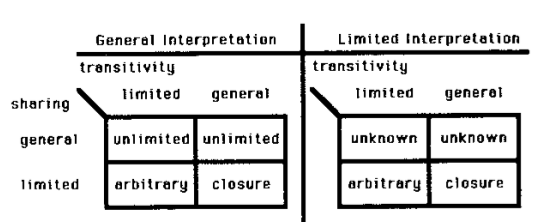
\includegraphics[width=0.60\textwidth]{figure/fig5.png}
    \caption{Limits of viral infection} 
    \label{fig5}
\end{figure} 







